% pdflatex rff-times.tex && rm *.aux *.log
% pdftoppm rff-times.pdf -rx 500 -ry 500 rff-times -png

\documentclass[varwidth]{standalone}
\usepackage{pgfplots}
\usepackage{graphicx}
\begin{document}

\resizebox{0.95\columnwidth}{!} {
% BIRD
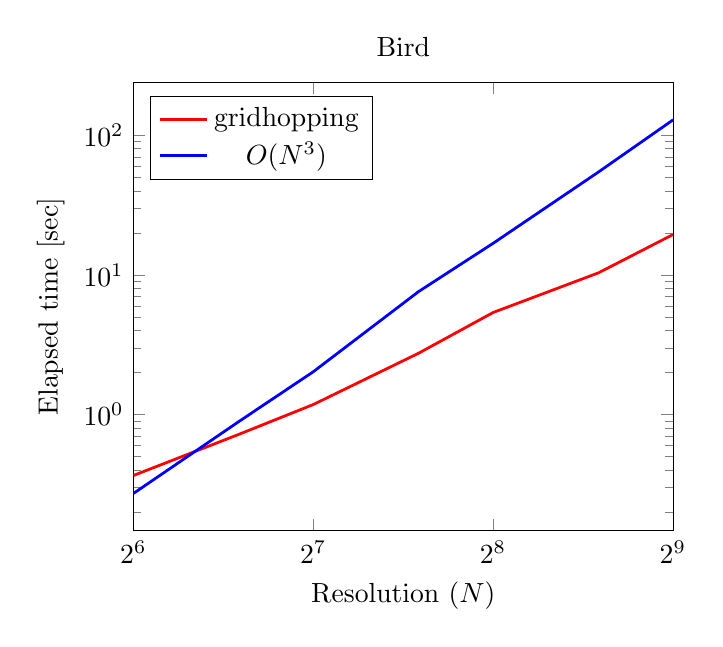
\begin{tikzpicture}
\begin{axis} [
	title=Bird,
	ymode=log,
	xlabel={Resolution ($N$)},
	ylabel={Elapsed time [sec]},
	xmin=64, xmax=512,
	xmode=log, log basis x=2,
	legend pos=north west
]
		\addplot[color=red, line width=1]
			coordinates {
				(64.000000, 0.367000)(96.000000, 0.722000)(128.000000, 1.182000)(192.000000, 2.751000)(256.000000, 5.388000)(384.000000, 10.344000)(512.000000, 19.474000)
			};
		\addplot[color=blue, line width=1]
			coordinates {
				(64.000000, 0.273000)(96.000000, 0.891000)(128.000000, 2.030000)(192.000000, 7.596000)(256.000000, 16.860000)(384.000000, 54.486000)(512.000000, 128.772000)
			};
		\legend{gridhopping,$O(N^3)$}
\end{axis}
\end{tikzpicture}
% FROG
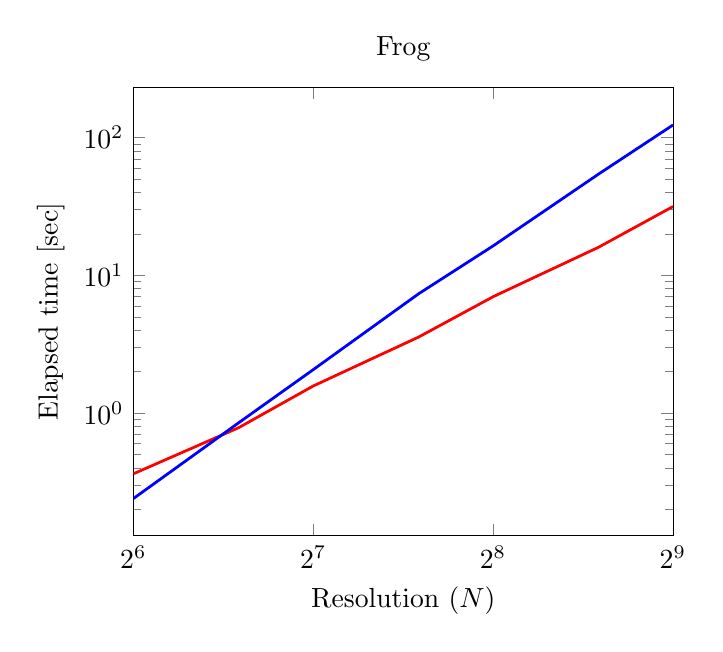
\begin{tikzpicture}
\begin{axis} [
	title=Frog,
	ymode=log,
	xlabel={Resolution ($N$)},
	ylabel={Elapsed time [sec]},
	xmin=64, xmax=512,
	xmode=log, log basis x=2,
	legend pos=north west
]
		\addplot[color=red, line width=1]
			coordinates {
				(64.000000, 0.363000)(96.000000, 0.784000)(128.000000, 1.575000)(192.000000, 3.561000)(256.000000, 6.999000)(384.000000, 15.959000)(512.000000, 31.579000)
			};
		\addplot[color=blue, line width=1]
			coordinates {
				(64.000000, 0.240000)(96.000000, 0.851000)(128.000000, 2.070000)(192.000000, 7.335000)(256.000000, 16.363000)(384.000000, 54.155000)(512.000000, 123.321000)
			};
\end{axis}
\end{tikzpicture}
% CATS
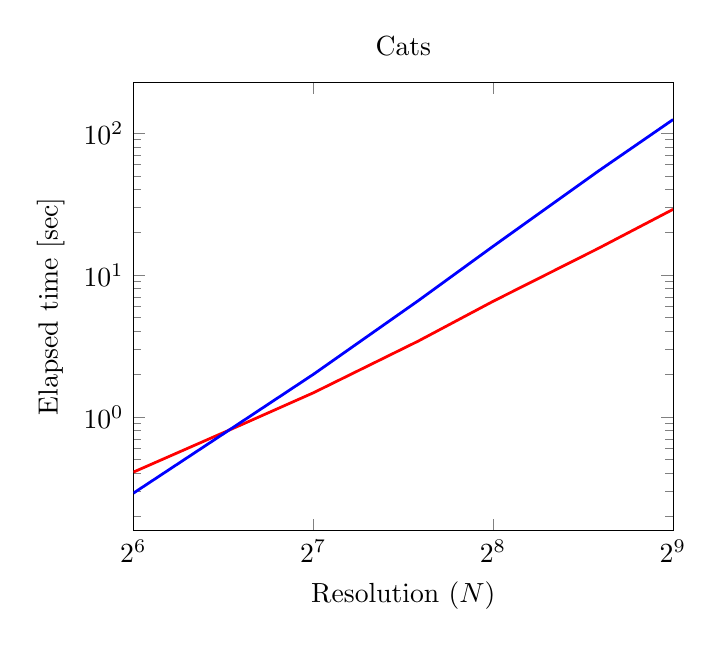
\begin{tikzpicture}
\begin{axis} [
	title=Cats,
	ymode=log,
	xlabel={Resolution ($N$)},
	ylabel={Elapsed time [sec]},
	xmin=64, xmax=512,
	xmode=log, log basis x=2,
	legend pos=north west
]
		\addplot[color=red, line width=1]
			coordinates {
				(64.000000, 0.408000)(96.000000, 0.863000)(128.000000, 1.477000)(192.000000, 3.427000)(256.000000, 6.528000)(384.000000, 15.405000)(512.000000, 29.014000)
			};
		\addplot[color=blue, line width=1]
			coordinates {
				(64.000000, 0.290000)(96.000000, 0.894000)(128.000000, 1.993000)(192.000000, 6.610000)(256.000000, 15.943000)(384.000000, 53.994000)(512.000000, 124.544000)
			};
\end{axis}
\end{tikzpicture}
}
\\
\resizebox{0.95\columnwidth}{!} {
% BUNNY
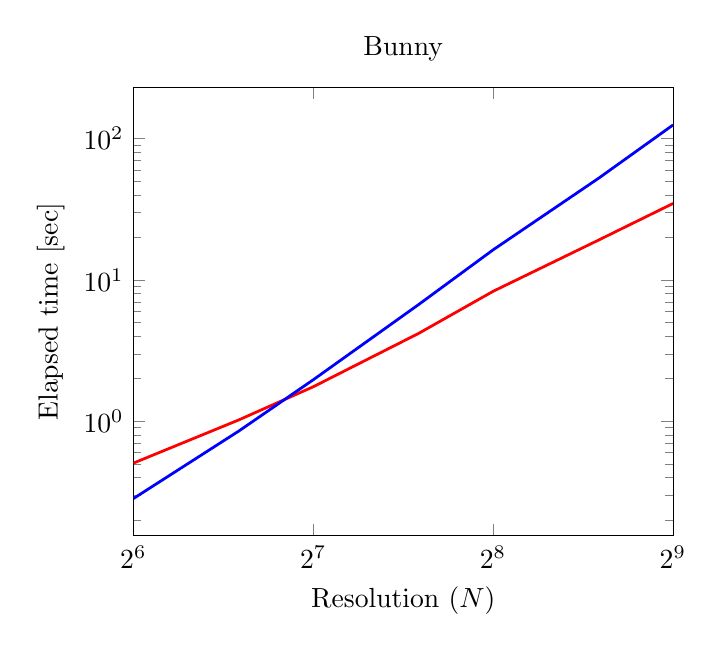
\begin{tikzpicture}
\begin{axis} [
	title=Bunny,
	ymode=log,
	xlabel={Resolution ($N$)},
	ylabel={Elapsed time [sec]},
	xmin=64, xmax=512,
	xmode=log, log basis x=2,
	legend pos=north west
]
		\addplot[color=red, line width=1]
			coordinates {
				(64.000000, 0.506000)(96.000000, 1.022000)(128.000000, 1.757000)(192.000000, 4.186000)(256.000000, 8.326000)(384.000000, 19.145000)(512.000000, 34.825000)
			};
		\addplot[color=blue, line width=1]
			coordinates {
				(64.000000, 0.284000)(96.000000, 0.852000)(128.000000, 1.970000)(192.000000, 6.696000)(256.000000, 16.372000)(384.000000, 52.399000)(512.000000, 125.197000)
			};
\end{axis}
\end{tikzpicture}
% MUSHROOMS
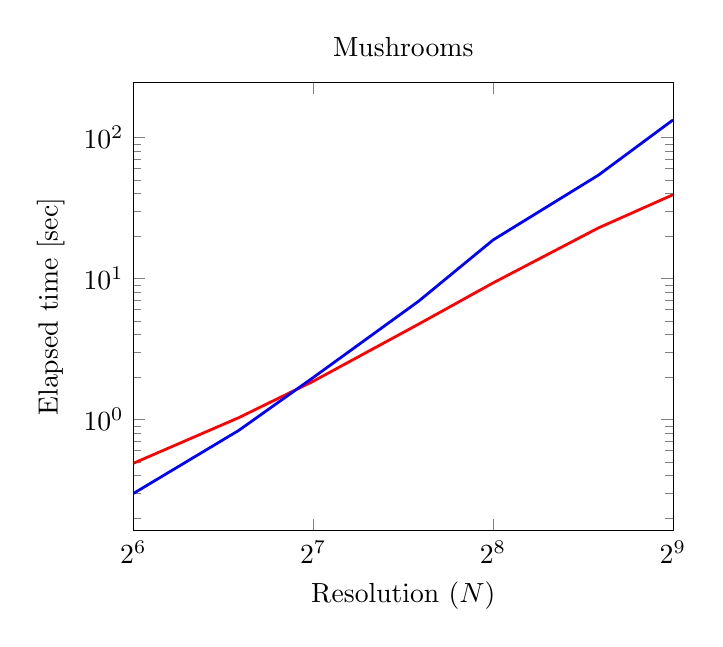
\begin{tikzpicture}
\begin{axis} [
	title=Mushrooms,
	ymode=log,
	xlabel={Resolution ($N$)},
	ylabel={Elapsed time [sec]},
	xmin=64, xmax=512,
	xmode=log, log basis x=2,
	legend pos=north west
]
		\addplot[color=red, line width=1]
			coordinates {
				(64.000000, 0.488000)(96.000000, 1.027000)(128.000000, 1.865000)(192.000000, 4.734000)(256.000000, 9.300000)(384.000000, 22.810000)(512.000000, 39.267000)
			};
		\addplot[color=blue, line width=1]
			coordinates {
				(64.000000, 0.298000)(96.000000, 0.834000)(128.000000, 1.984000)(192.000000, 6.883000)(256.000000, 18.771000)(384.000000, 54.037000)(512.000000, 133.349000)
			};
\end{axis}
\end{tikzpicture}
% WHALE
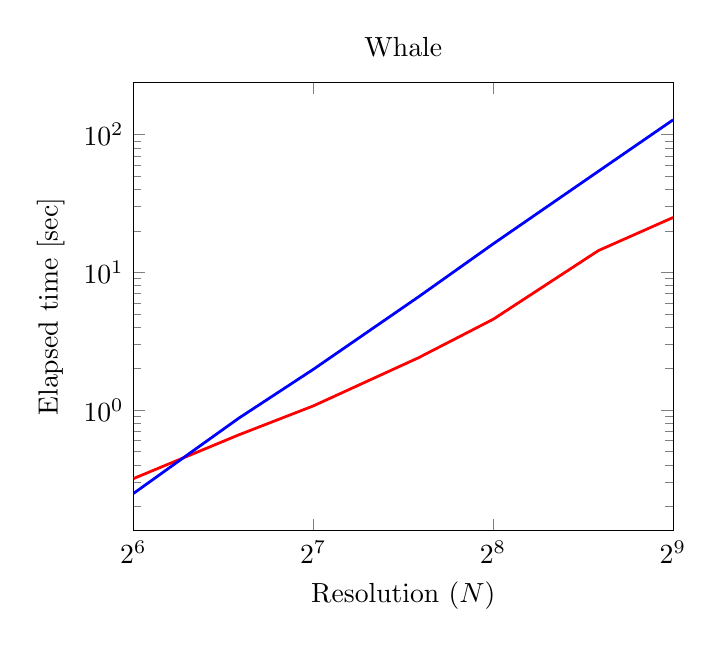
\begin{tikzpicture}
\begin{axis} [
	title=Whale,
	ymode=log,
	xlabel={Resolution ($N$)},
	ylabel={Elapsed time [sec]},
	xmin=64, xmax=512,
	xmode=log, log basis x=2,
	legend pos=north west
]
		\addplot[color=red, line width=1]
			coordinates {
				(64.000000, 0.318000)(96.000000, 0.660000)(128.000000, 1.072000)(192.000000, 2.398000)(256.000000, 4.563000)(384.000000, 14.381000)(512.000000, 25.014000)
			};
		\addplot[color=blue, line width=1]
			coordinates {
				(64.000000, 0.248000)(96.000000, 0.872000)(128.000000, 1.976000)(192.000000, 6.639000)(256.000000, 16.100000)(384.000000, 54.161000)(512.000000, 127.936000)
			};
\end{axis}
\end{tikzpicture}
}

\end{document}
